\chapter{Coordinate Geometry}

\section{Introduction}
Many of you have encountered some form of coordinate geometry in high school. For instance, the "standard" way to visualize a graph e.g. $f(x)=x^2$ is to visualize the points in 2-D space $(x,y)$ where $y=x^2$. We give an demonstration in Python code.

\begin{lstlisting}[language=Python]
import matplotlib.pyplot as plt
import numpy as np
X=np.array(range(-100,100)) #create list of numbers from -100 to 100
Y= X**2 #calculate the square of at each x
plt.plot(X,Y) #plot all the pairs of points in 2d plane
plt.xlabel('x')
plt.ylabel('y=x^2')
plt.title('Visualization of the "object"')
plt.show()
plt.show()
\end{lstlisting}
\begin{tikzpicture}
	\node (A) at (0,0) {$x$}
	\node (B) at (3,0) {$x^2$}
	\draw[->,thick]
	(A)--(B)
	node[midway,below] {the "graph" object} 
	\node(whitehead) at (8,0){
		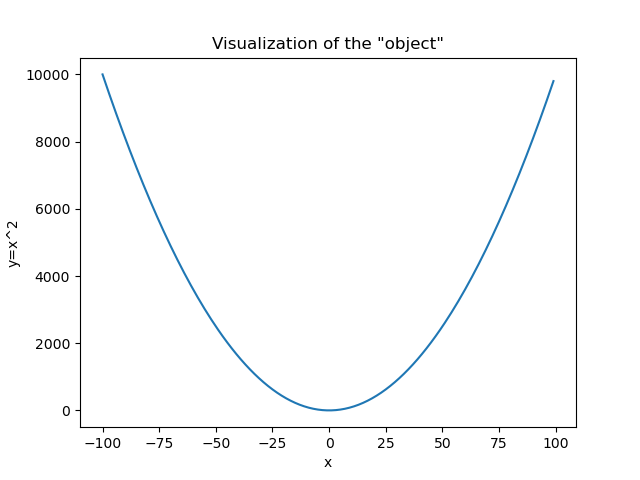
\includegraphics[width=0.6\textwidth]{coordinate_geometry/square_graph.png}
	}
\end{tikzpicture}


This is also known as the Cartesian plane, after Descartes who invented it in the 17th century.\\
\section{Visualization of geometric objects in the Cartesian plane}
The Cartesian plane allows us to describe shapes with equations and perform calculations with them. We first define the playing field (the Cartesian plane and higher dimensional analogues) and the players.
\definition{Real numbers}{
	The set of \textbf{real numbers}, denoted as $\mathbb{R}$, is (informally) the set of all the numbers that can be written out in decimal form.
}
\example{
The following are real numbers:
\begin{enumerate}
	\item The integers $0$, $\pm 1$, $\pm 2$, ...  
	\item Fractions in the form $\frac{a}{b}$, where $a$ and $b\neq 0$ are integers.
	\item Irrational numbers $\sqrt{2}$, $\pi$.
\end{enumerate}
}
\begin{remark}
	The set of real numbers is known as a \textbf{complete field}. The definition of a complete field will be swept under the rug, but it guarantees a few things. The most important property: We will not "escape" the set by performing operations, possibly infinitely many.
\end{remark}
\definition{N-dimensional space}{
	Let $n$ be a positive integer. We denote the \textbf{n-dimensional real space} to be $\mathbb{R}^n$, consisting of all the $n$-tuples $(x_1,x_2,x_3,...,x_n)$, where each $x_j$ is a real number. \\
	We call an $n$-tuple $(x_1,...,x_n)$ a \textbf{point}, and two points $(x_1,...,x_n)$ and $(y_1,...,y_n)$ are equal if $x_j=y_j$ for all $j$-th entries of the tuples.
}
\begin{remark}
	We sometimes use $\mathbf{x}$ to denote the tuple $(x_1,...,x_n)$ to make notation cleaner.
\end{remark}
\subsection{Lines}
Now that we have introduced the playing field of n-dimensional space, we can start translating the axioms of euclidean geometry to this coordinate system.
\definition{Lines}{
	In euclidean geometry, a line is defined by two points. We let $\mathbf{x},\mathbf{y} \in \mathbb{R}^n$. The \textbf{line} going from $\mathbf{x}$ to $\mathbf{y}$ is denoted $\overrightarrow{\mathbf{xy}}$.
}
What would this line look like? To get from $\mathbf{x}$ to $\mathbf{y}$, we have to traverse $y_1-x_1$ units in the first coordinate, $y_2-x_2$ units in the second, ..., $y_n-x_n$ in the last. We thus have a natural notation for the line $\overrightarrow{\mathbf{xy}}$.
\[
 \overrightarrow{\mathbf{xy}}=(y_1-x_1,y_2-x_2,...,y_n-x_n).
\]

This is very similar to a point as an n-tuple, but this is "spiritually" different to a point. This tuple represents the direction of line. One way to think of the correspondence between $(x_1,...,x_n)$ point and $(x_1,...,x_n)$ line is that $(x_1,...,x_n)$ line is the line connecting $(0,0,...0)$ to $(x_1,...,x_n)$ point.


\begin{tikzpicture}[node distance=2cm]
	
	\node  (A) at (0,0) {$(0,..,0)$}
	\node  (B) at (9.5,1) {point $(x_1,...,x_n)$}
	\draw[thick, ->]
	(A) -- (B) 
	node[midway, below right] {line $(x_1,..,x_n)$};
\end{tikzpicture}
We now formalize this observation.

\proposition{
Lines are \textbf{translation invariant}.
That is, let $(x_1,...,x_n)$, $(y_1, ..., y_n)\in \mathbb{R}^n$, and $n$ real numbers $c_1, c_2,...,c_n\in \mathbb{R}$.
\\
The line going from $(x_1,...,x_n)$ to $(y_1,...y_n)$ is equal to the line going from $(x_1+c_1,x_2+c_2,...,x_n+c_n)$ to $(y_1+c_1,y_2+c_2,...,y_n+c_n)$ in each of the entries.
}


\subsection{Operation with lines}
We need to translate a few more things from euclidean geometry.
\definition{Length of line}{
	
}
\exercises
